\section{Implementation}\label{sec:implementation}
In this chapter, I am going to describe the implementation process and its related details of the demonstrator in detail. Section \ref{subsec:coredetails} describes the overview of the implementation of the demonstrator with component, activity, and sequence diagrams. This is then followed by the detail description of the implementation steps involved in each layer i.e., Model, View, and Controller in Section \ref{subsec:imple_layers}. At last, Section \ref{subsec:implechallenges} describes the challenges that I faced while implementing the entire framework and its components.

\subsection{Core Details}\label{subsec:coredetails}
This section provides an overview of the implementation steps involved with the demonstrator. First, I introduce the components of the tool and their interconnection. Then, I describes the general workflow of the tool by showing in which order which activities are executed. Finally, the communication between the components is presented.

\subsubsection{Component Architecture}\label{subsubsec:component}
The architecture has three components to signify Model-View-Controller (MVC) pattern. Figure~\ref{fig:Component_Diagram} describes the high-level architecture of the tool in form of a component diagram.

\begin{sidewaysfigure}
	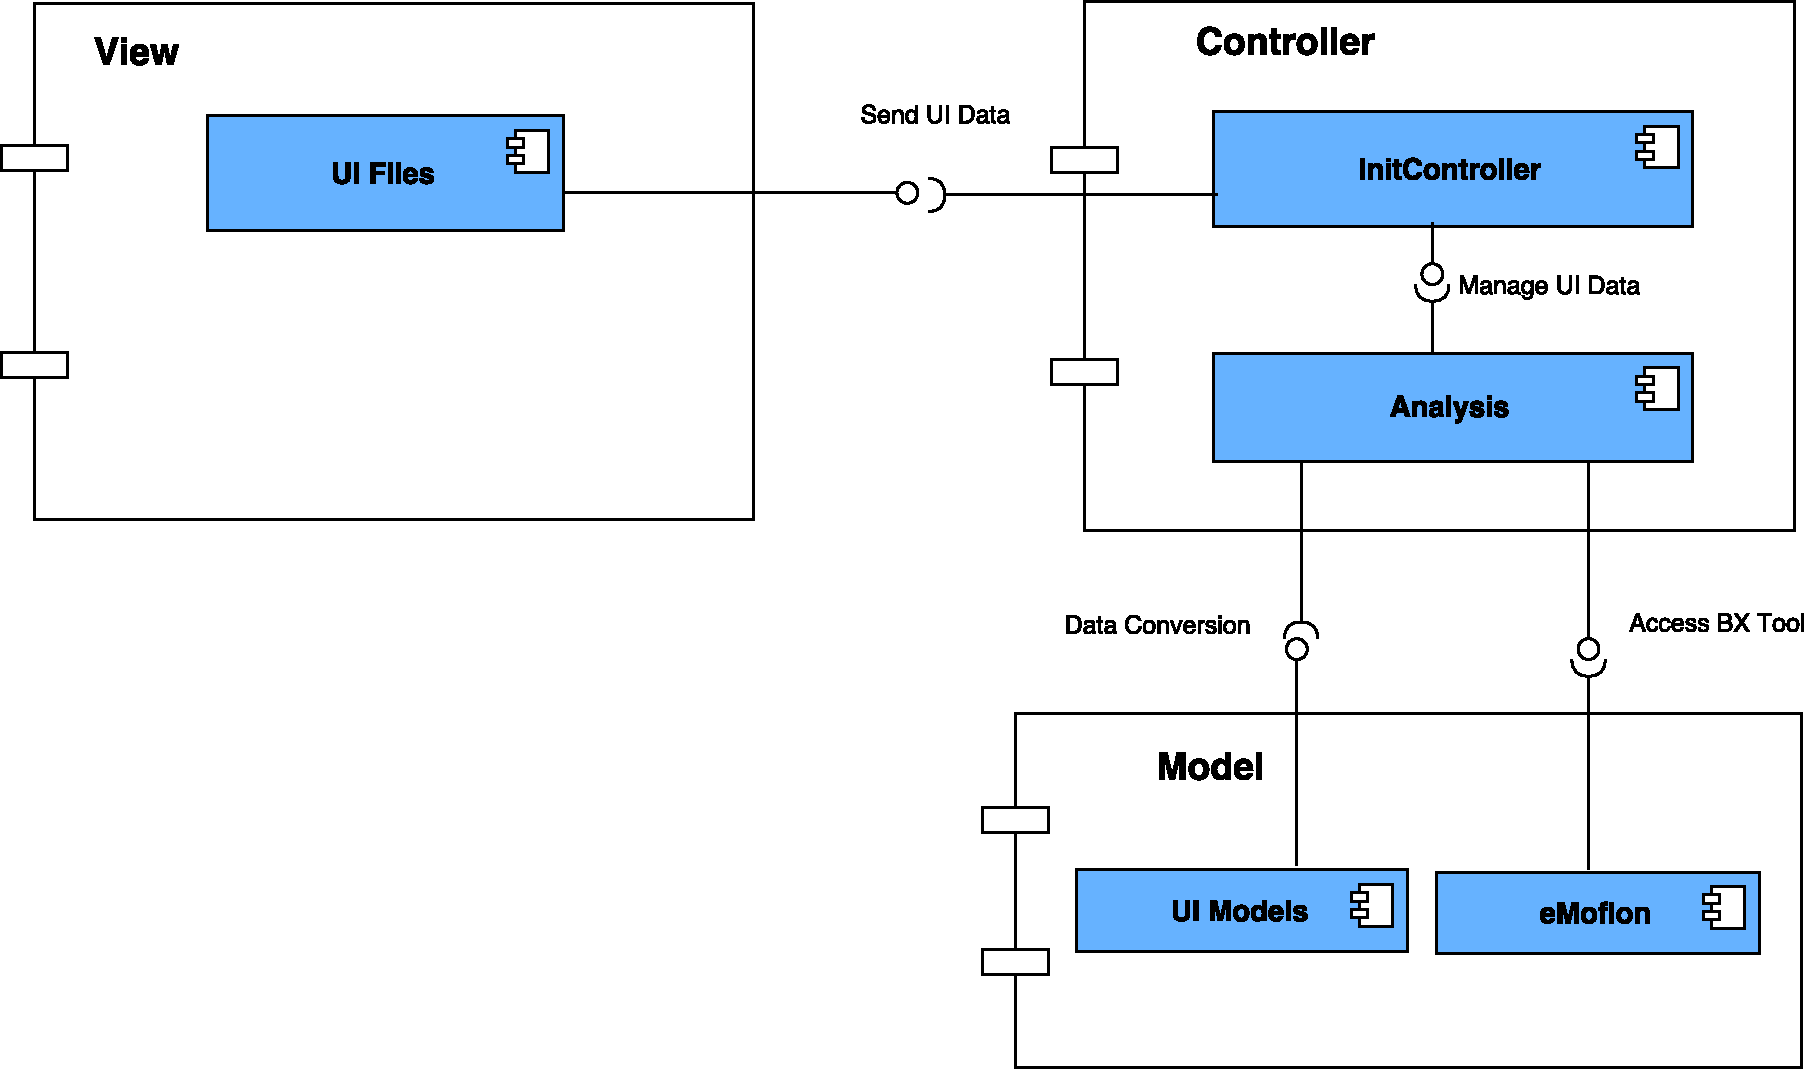
\includegraphics[width=1\textwidth]{figures/Component_Diagram}
	\caption{Component Diagram of Demon-BX Tool}
	\label{fig:Component_Diagram}
\end{sidewaysfigure}

On the top, \texttt{View} (Web Browser) component is present which contains a graphical user interface and functionalities that belong to the user. With the changes on \texttt{View} component, data are being provided through interface \texttt{IDoAnalysis} to the \texttt{Controller} component and after the calculations are done, the results are sent back to the \texttt{View} through interface \texttt{IProvideResults}. Both \texttt{View} and \texttt{Controller} resides on the same machine. \texttt{Model} (Bx Tool) component encapsulates and manages the state of all models by communication with the \texttt{Controller} through interface \texttt{IRules}.

\subsubsection{General Workflow}\label{subsubsec:generalworkflow}

\begin{figure}
	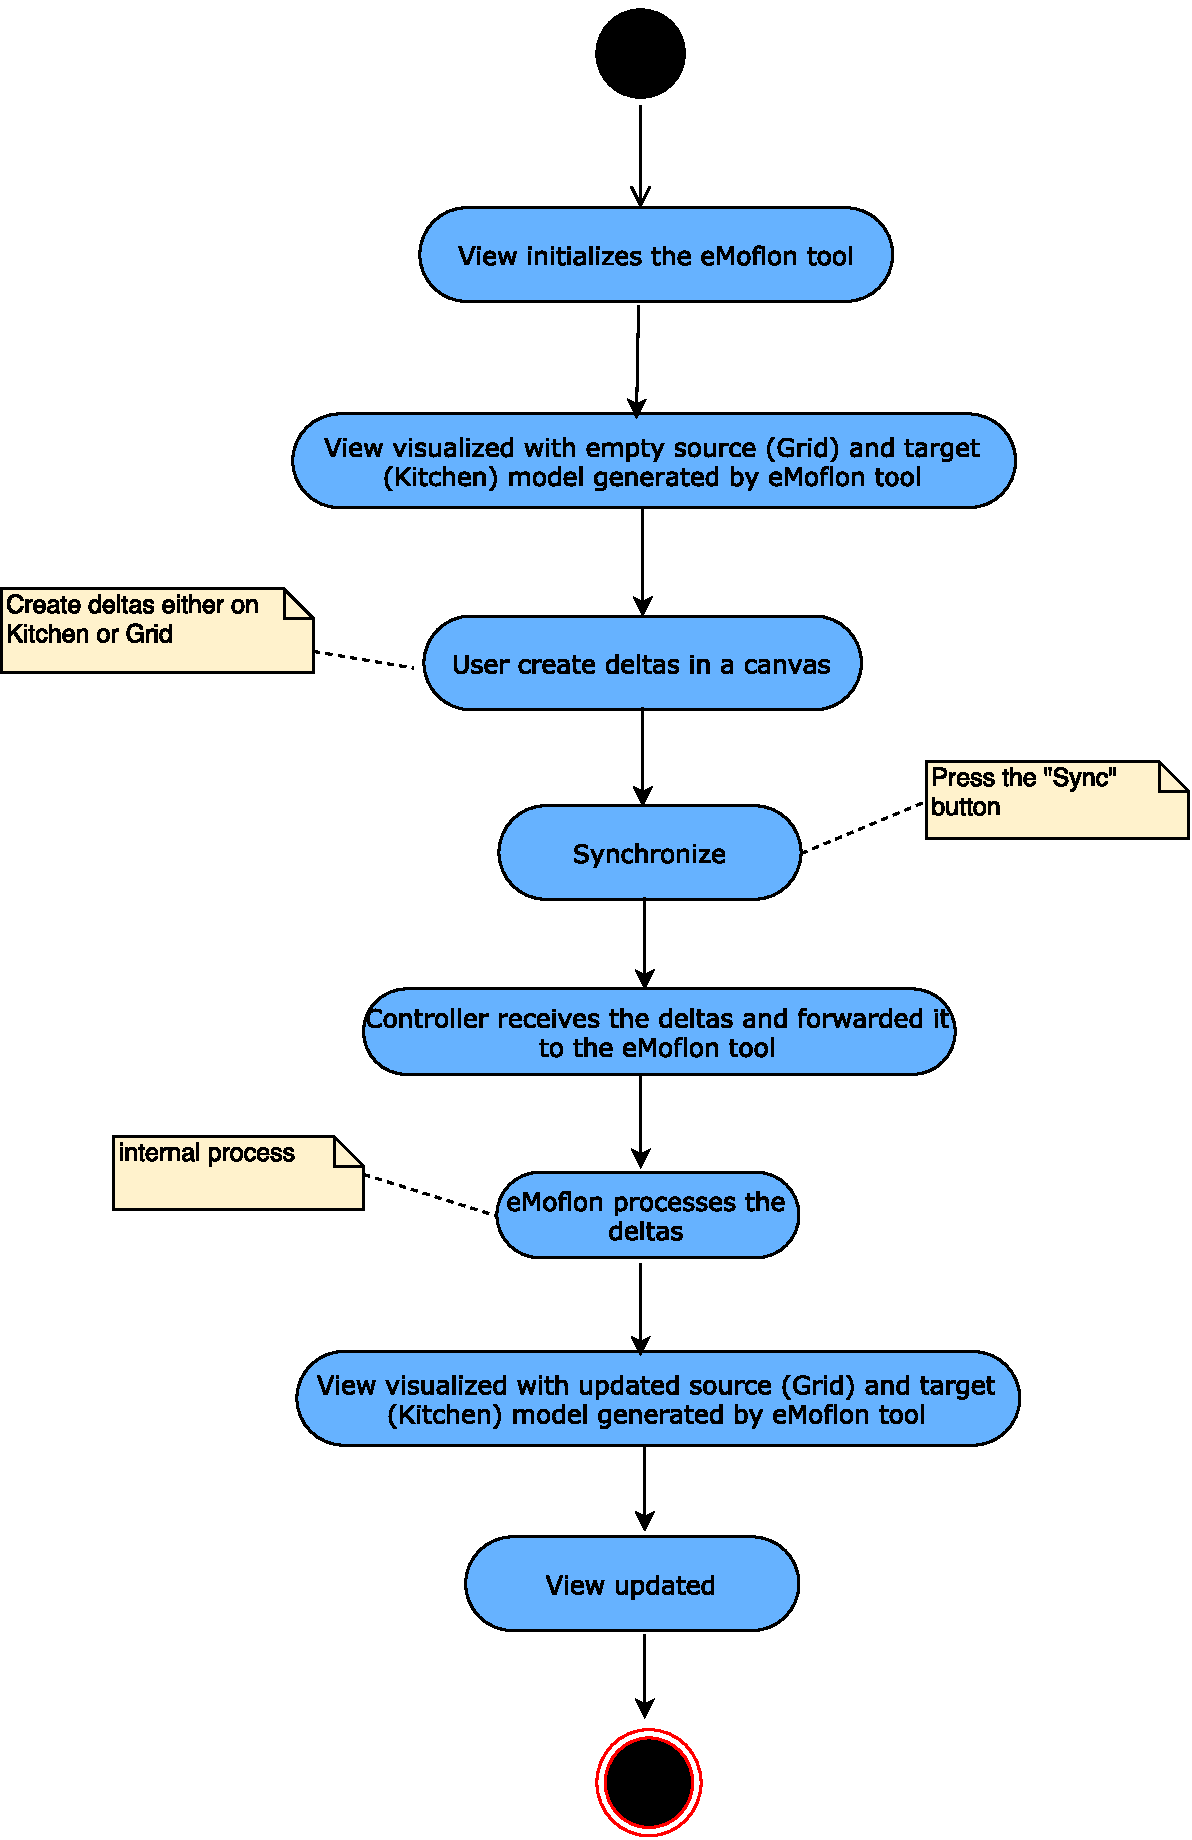
\includegraphics[width=0.9\textwidth]{figures/Activity_Diagram}
	\caption{Activity Diagram for General Workflow of Demon-BX Tool}
	\label{fig:Activity_Diagram}
\end{figure}

\subsubsection{Interaction between the Components}\label{subsubsec:componentinteraction}

\begin{figure}
	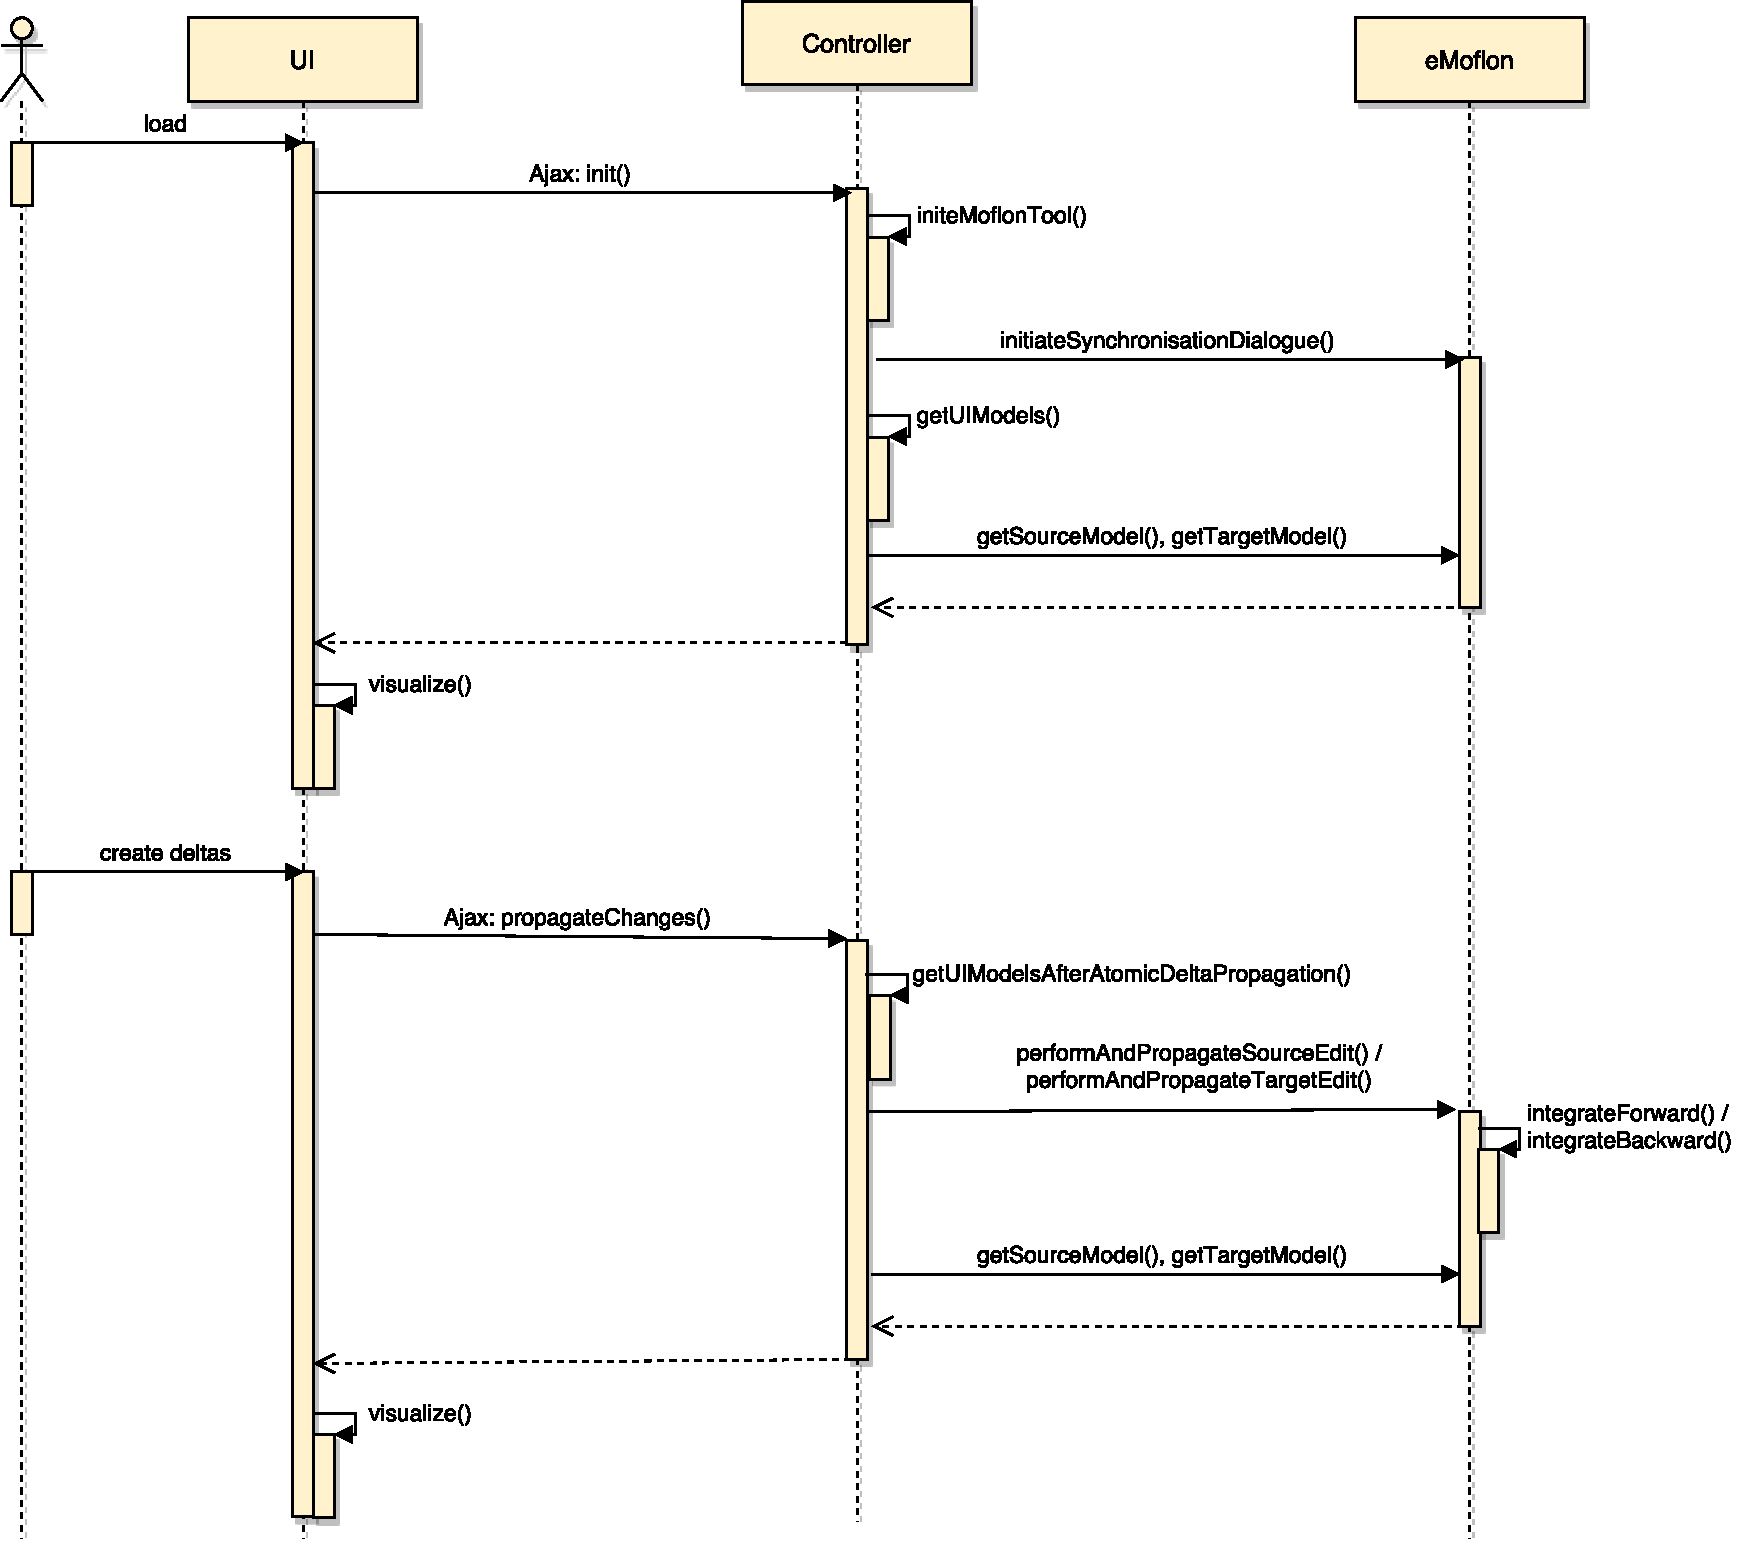
\includegraphics[width=1\textwidth]{figures/Sequence_Diagram}
	\caption{High Level Sequence Diagram of Demon-BX Tool}
	\label{fig:Sequence_Diagram}
\end{figure}

\subsection{Architecture Layers}\label{subsec:imple_layers}
This section describes each architecture layers i.e., Model, View, and Controller in detail from implementation point of view.

\subsubsection{Model}\label{subsubsec:imple_model}
\paragraph{Transformation Rules}

\subsubsection{View}\label{subsubsec:imple_view}

\begin{figure}
	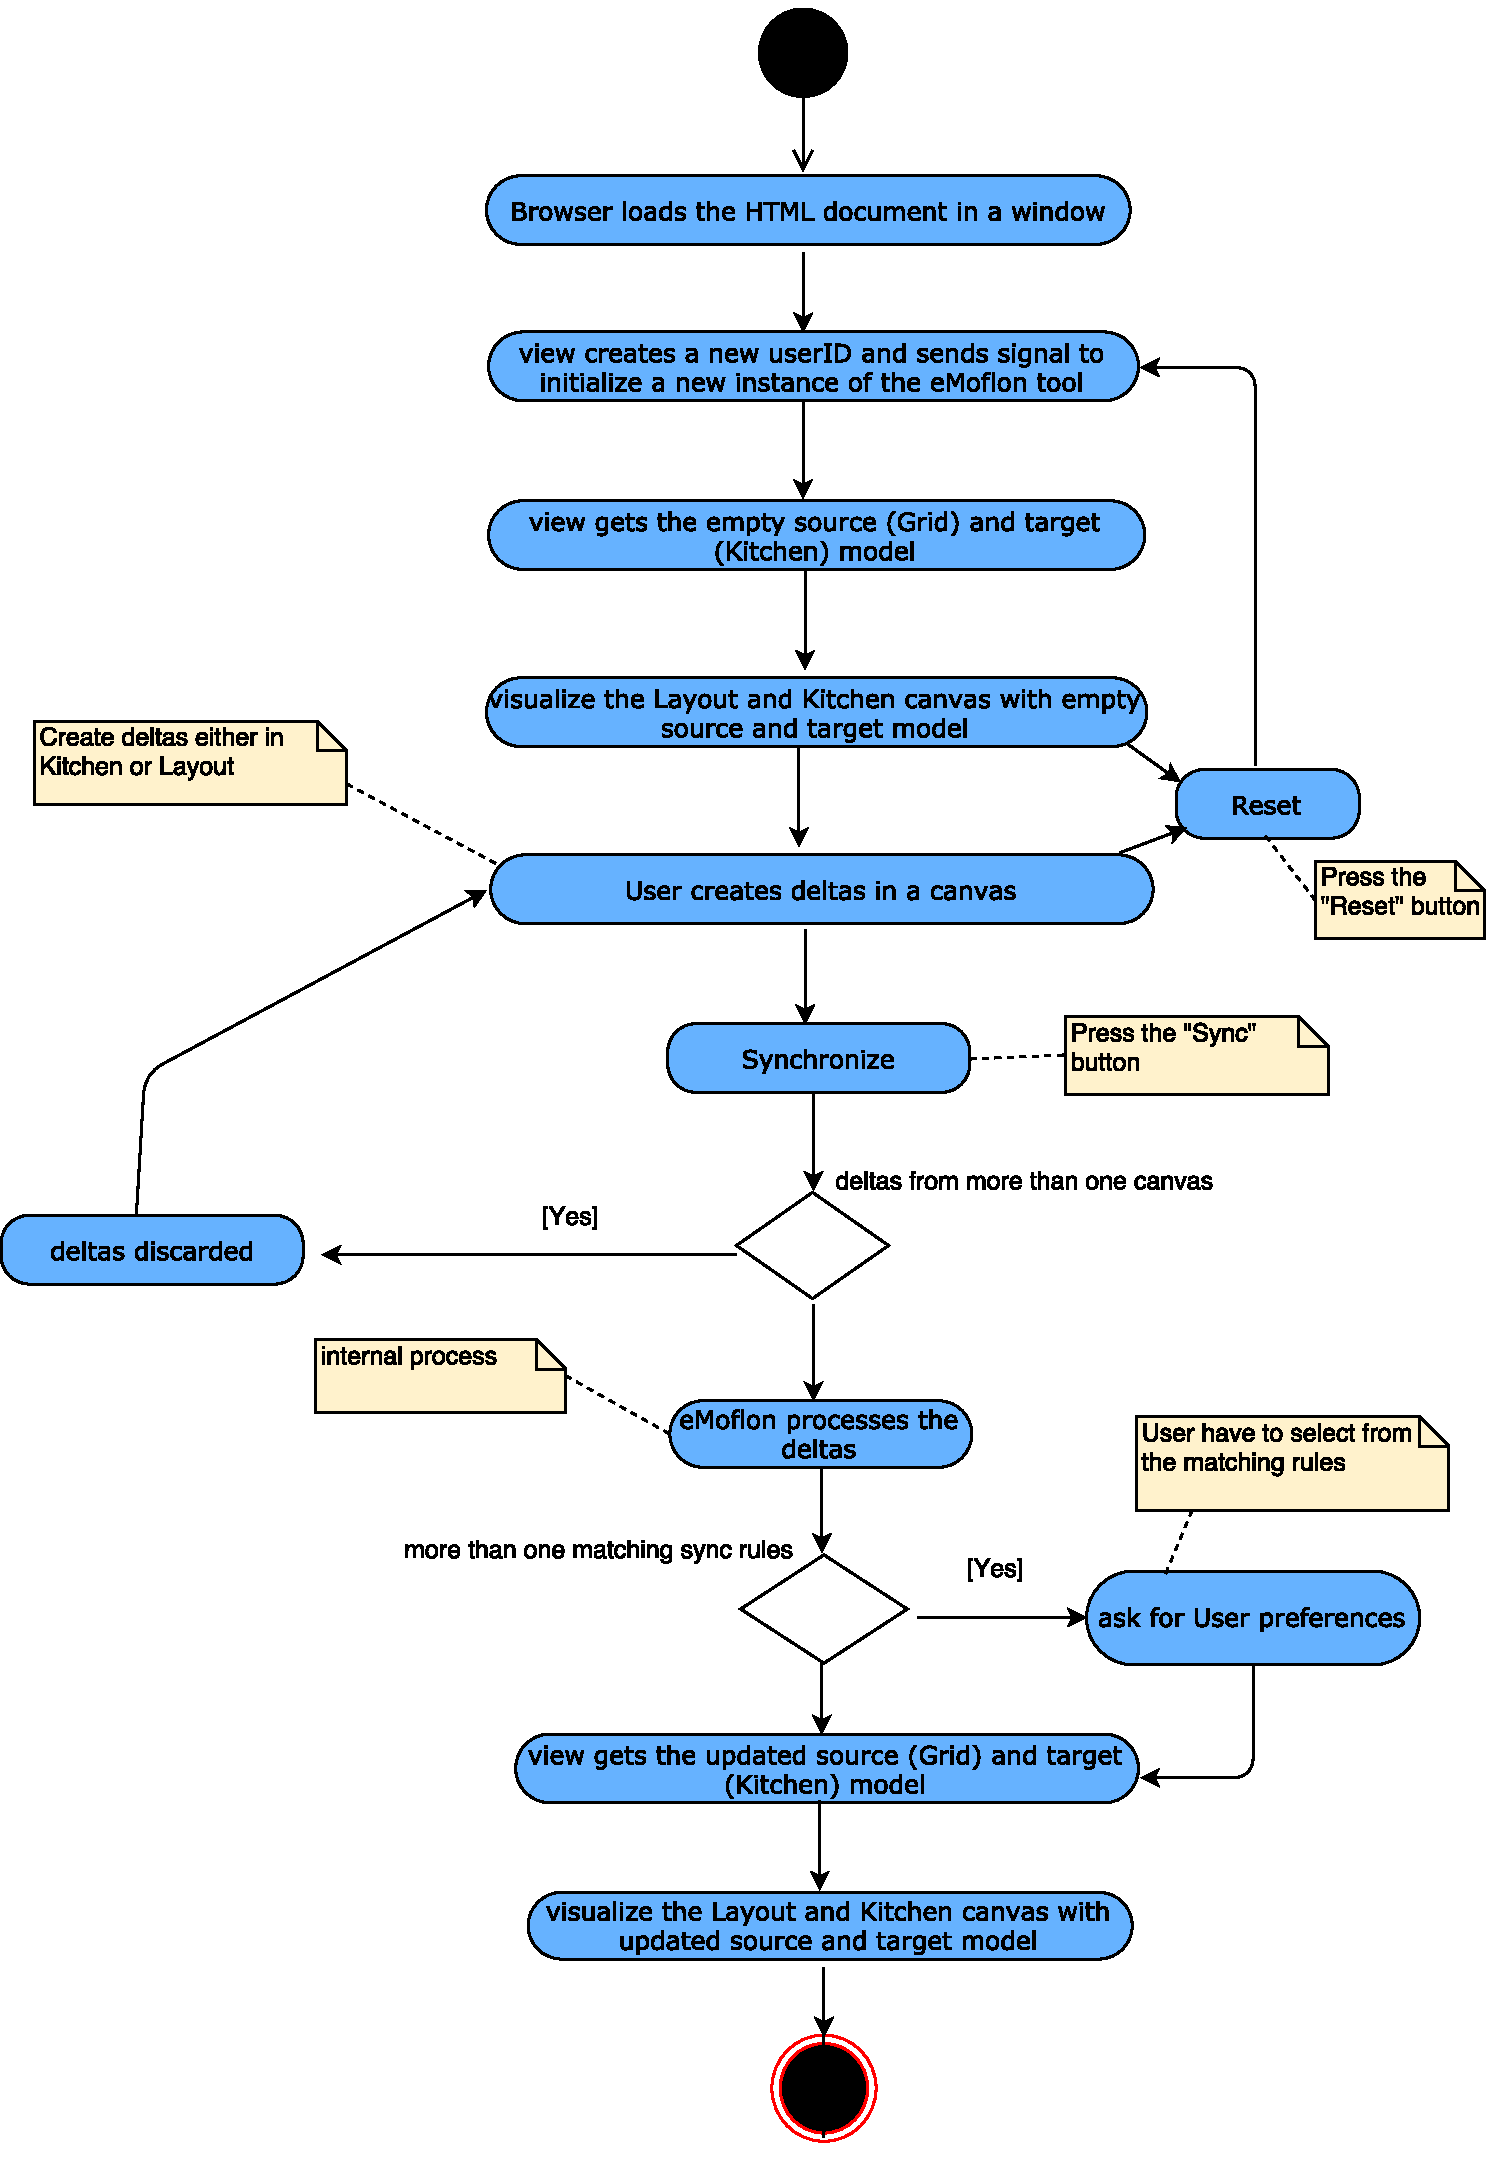
\includegraphics[width=0.9\textwidth]{figures/Activity_Diagram_View}
	\caption{Activity Diagram for View}
	\label{fig:Activity_Diagram_View}
\end{figure}

\subsubsection{Controller}\label{subsubsec:imple_controller}
controller and helper - how servlet is implemented with actual class name and func.

\subsection{Challenges}\label{subsec:implechallenges}
During the entire implementation process as explained in previous sections of this chapter, I came across a few challenges. This section describes them in detail.

\paragraph{Bx Tool}
selecting the type of delta (refer def.)
implementing atomic deltas to track successful/failed changes translation. 
User Choice Selection -- interupting the tool inbetween and start the process again

\paragraph{UI Implementation}
Designing the user interactions with high-level view was relatively easy as user have to deal with the objects with actions such as, mouse movements and button clicks. But, the real challenge was to handle the user interactions in low-level view's block structure. In low-level view, only addition and removal of objects are allowed and objects will be shown by unique colors. 

\paragraph{User Choice Selection}

\paragraph{Handling Multiple User Request}
 



